\chapter{Solving}

\chapter{Problems}

% introduction
\section{Problems}

To define a problem is defining a class at the same time.

To understand a problem is to know how to check whether one solution is correct or not.
\subsection{Verifying versus Searching}


% types of problems
\section{Types of Problems}
\subsection{Computational Problems}
\subsection{Learning Problems}
\subsection{Generic Problems}

% definition and properties of techniques
\section{Techniques}
The Classification of Techniques is a core concept in daily life.
\begin{figure}
  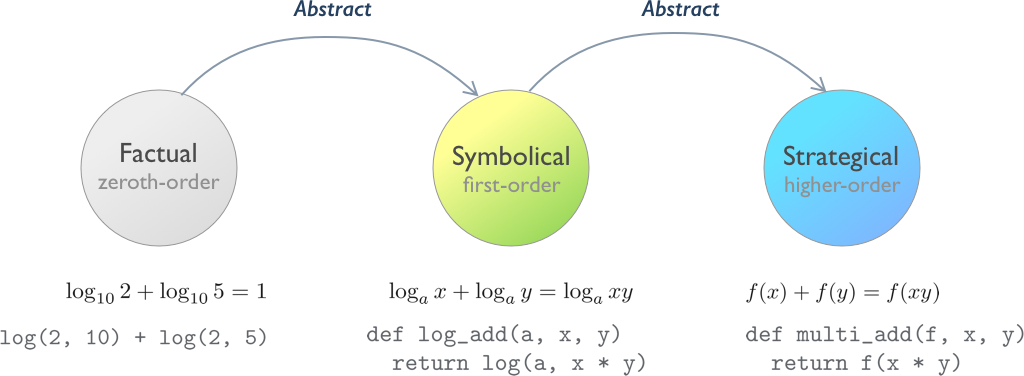
\includegraphics[width=\linewidth]{img/abstract-levels.png}
  \caption{Abstraction Levels}
  \label{fig:abstract-levels}
\end{figure}
\subsection{Robustness of Techniques}
\subsection{Frequency of Usage}
\subsection{Ad-Hoc versus Generic}
One phenominon that I experience a lot is the way people don't distinguish the difference between a ad-hoc technique and a generic technique. When a teacher or a guy present a way to solve a specific problem, few people will appreciate the robustness of this technique, that how well can you transfer your ability on this learning to another situations. But because of their inability to distinguish hardness and robustness, that leads to a dangerous place, that you have to learn too much techniques to cope with every problems, but you don't have enough time for learning these. And the teacher may think by doing an ad-hoc problem will lead to a better understanding for a more generic solving ability, which is vague. You don't learn too much on ad-hoc problems. You only know how to solve it in a nearby situations. The overall hint on a more generic solving strategies are often weak to recognize.

People don't know how to appreciate the robustness of techniques. Only can they find the dramatic changes of events. Even you simply press the button, you believe the underlining changes belongs to your smartness, well the main reason is the engineering behind the scene to smooth the user experience.
\subsection{Intensity of Signal}
\subsection{Trainability of Techniques}
Both the solving radius and the applicability.

% types of techniques
\section{Types of Techniques}
\subsection{Factual Techniques}
\subsection{Algorithmic Techniques}
\subsection{Strategic Techniques}
\subsection{Generic Techniques}
\subsection{Expansion Techniques}


\chapter{Problems}

% introduction
\section{Problems}

To define a problem is defining a class at the same time.

To understand a problem is to know how to check whether one solution is correct or not.
\subsection{Verifying versus Searching}


% types of problems
\section{Types of Problems}
\subsection{Computational Problems}
\subsection{Learning Problems}
\subsection{Generic Problems}

% definition and properties of techniques
\section{Techniques}
The Classification of Techniques is a core concept in daily life.
\begin{figure}
  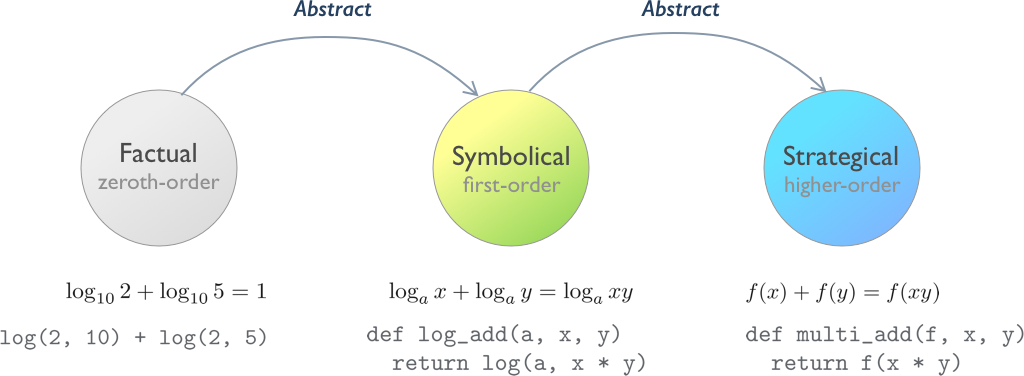
\includegraphics[width=\linewidth]{img/abstract-levels.png}
  \caption{Abstraction Levels}
  \label{fig:abstract-levels}
\end{figure}
\subsection{Robustness of Techniques}
\subsection{Frequency of Usage}
\subsection{Ad-Hoc versus Generic}
One phenominon that I experience a lot is the way people don't distinguish the difference between a ad-hoc technique and a generic technique. When a teacher or a guy present a way to solve a specific problem, few people will appreciate the robustness of this technique, that how well can you transfer your ability on this learning to another situations. But because of their inability to distinguish hardness and robustness, that leads to a dangerous place, that you have to learn too much techniques to cope with every problems, but you don't have enough time for learning these. And the teacher may think by doing an ad-hoc problem will lead to a better understanding for a more generic solving ability, which is vague. You don't learn too much on ad-hoc problems. You only know how to solve it in a nearby situations. The overall hint on a more generic solving strategies are often weak to recognize.

People don't know how to appreciate the robustness of techniques. Only can they find the dramatic changes of events. Even you simply press the button, you believe the underlining changes belongs to your smartness, well the main reason is the engineering behind the scene to smooth the user experience.
\subsection{Intensity of Signal}
\subsection{Trainability of Techniques}
Both the solving radius and the applicability.

% types of techniques
\section{Types of Techniques}
\subsection{Factual Techniques}
\subsection{Algorithmic Techniques}
\subsection{Strategic Techniques}
\subsection{Generic Techniques}
\subsection{Expansion Techniques}

How intimidating it is for a newcomer to a new city.

\section{Principle of Heuristics}
\subsection{Computational Cost Saving}

\section{The Analogy of City Exploration}

Since to solve is to search, searching is basically exploring your searchable area.

You start with a newly assigned treasure hunt game. You start you search by going through the known routes, following the familiar signposts, try the nearby stores to save your energy, you find a famous gathering place like a museuem or a park.

You start to find the easter egg by visiting the hinted places, and you get there by some known and familiar routes, you can search nearby the hinted places, since you know how to get there and assume you can find there will be considered as being lucky. Sometimes you have to find your own routes by noticing the signposts. And since you might visit the city multiple times, you will gradually remember the notable objects. When you on a road, you will automatically complete the routes without thinking or even chatting with others, until a puzzled crossroad is encountered.

Let's compare the solving route as how much roads you have to travel. And the fluency of your technique mastering is a value of resistance, low value with well trained, and high for poor practice. That might be the case in our brain that the smooth of a chunk is basically the electric current with higher value. And the brain choose load through those low resistance route to save computation energy.

\begin{figure}
  \centerline{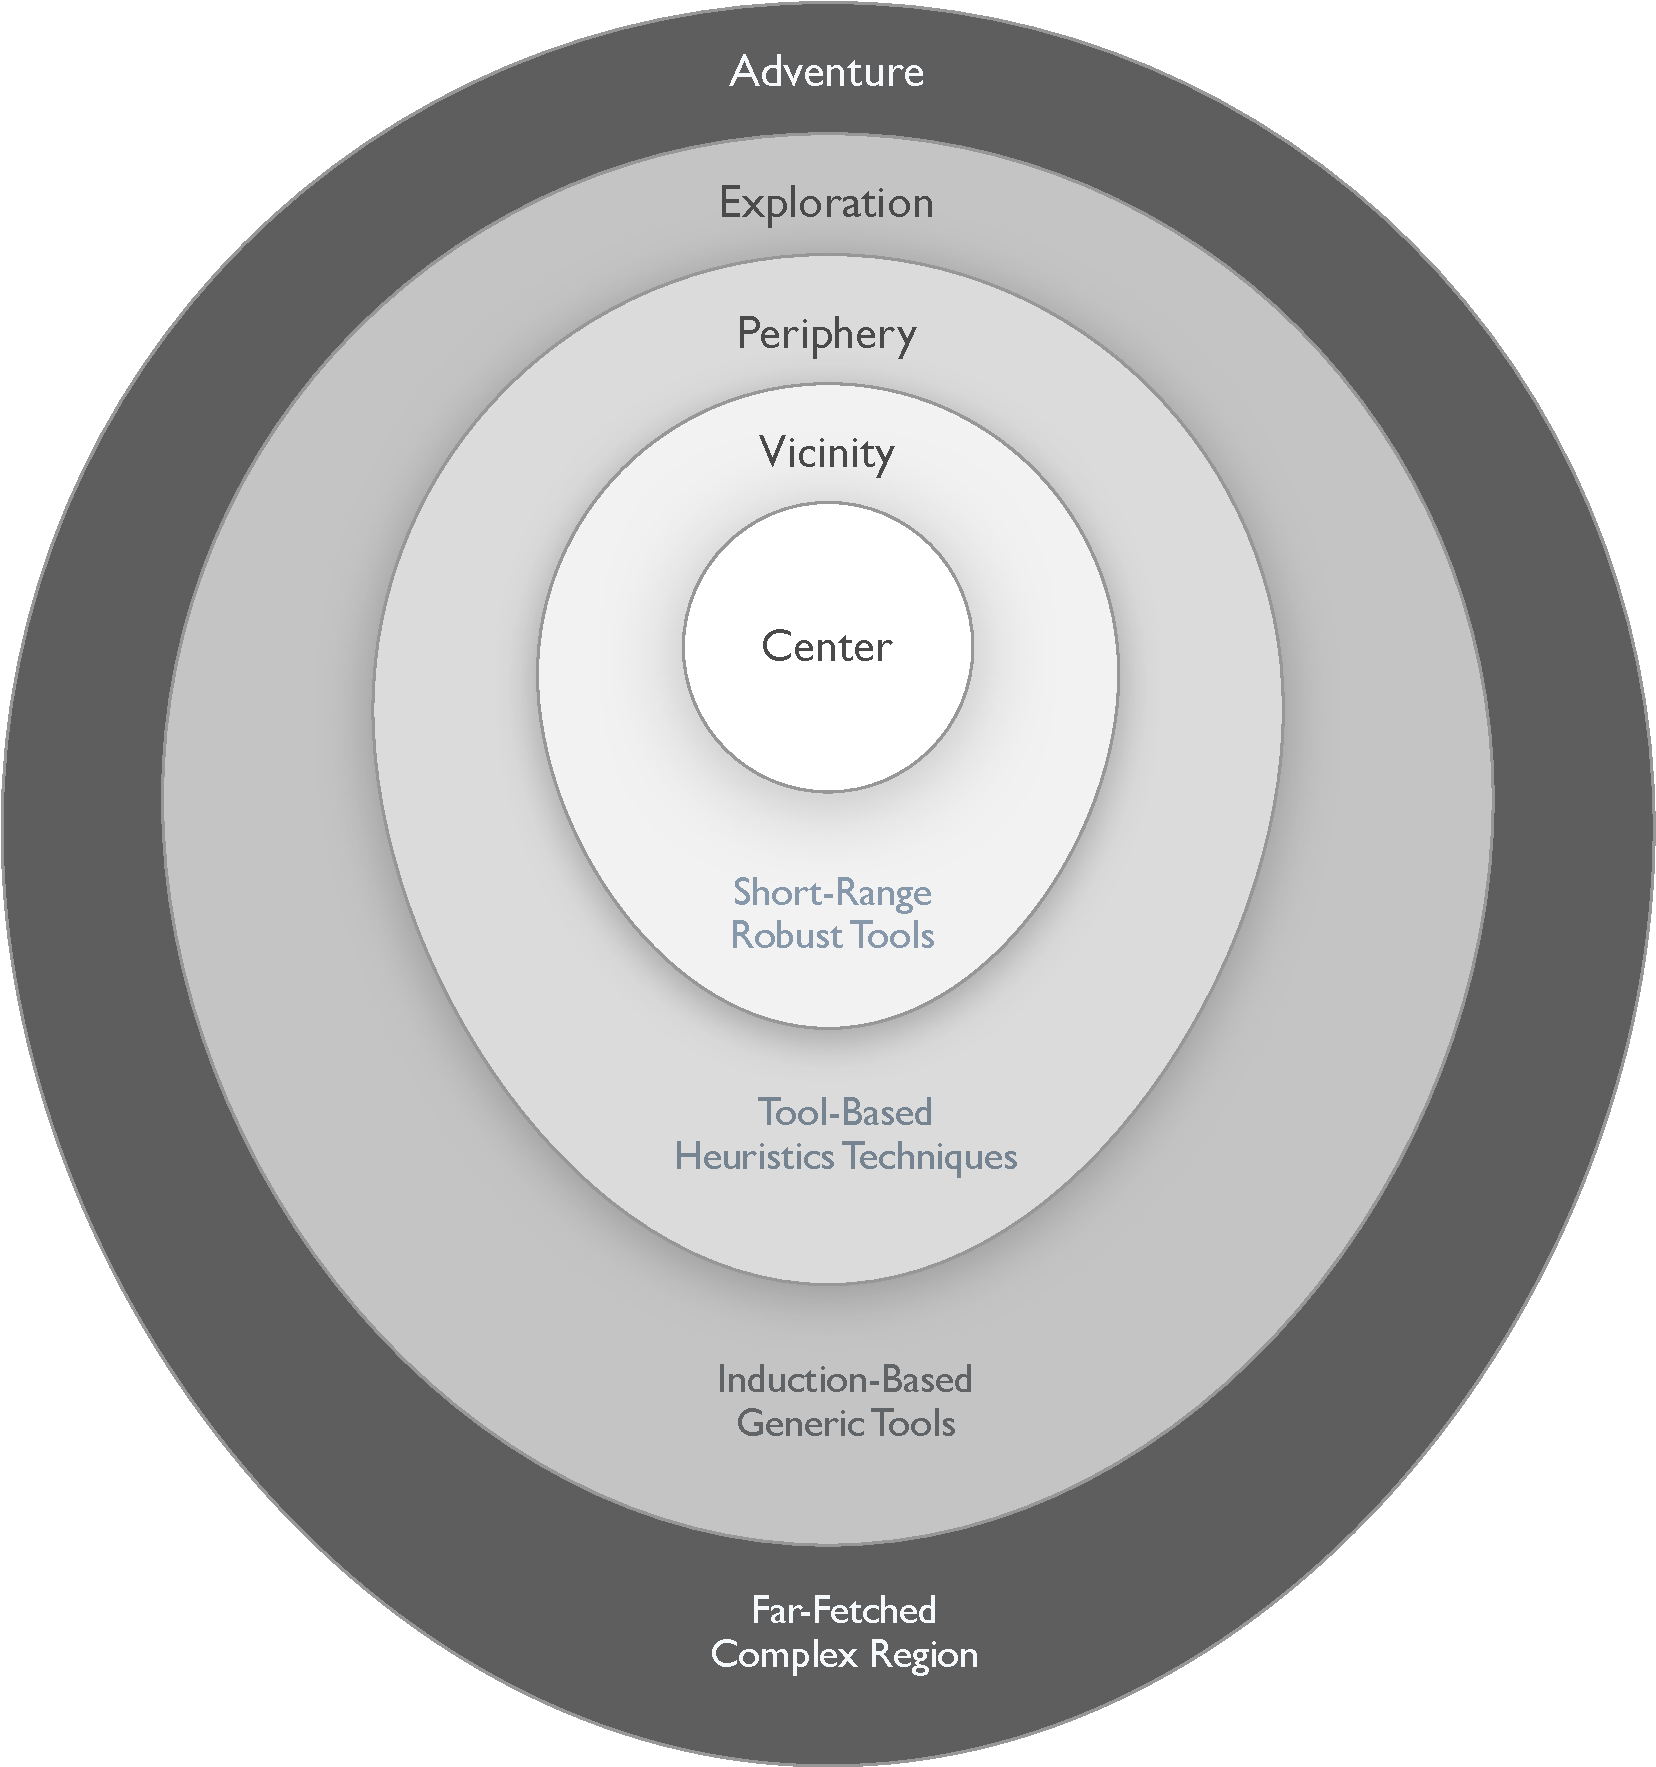
\includegraphics[width=1.2\linewidth]{img/range.pdf}}
  \caption{Types of Transformation}
  \label{fig:range}
\end{figure}


\chapter{Problems}

% introduction
\section{Problems}

To define a problem is defining a class at the same time.

To understand a problem is to know how to check whether one solution is correct or not.
\subsection{Verifying versus Searching}


% types of problems
\section{Types of Problems}
\subsection{Computational Problems}
\subsection{Learning Problems}
\subsection{Generic Problems}

% definition and properties of techniques
\section{Techniques}
The Classification of Techniques is a core concept in daily life.
\begin{figure}
  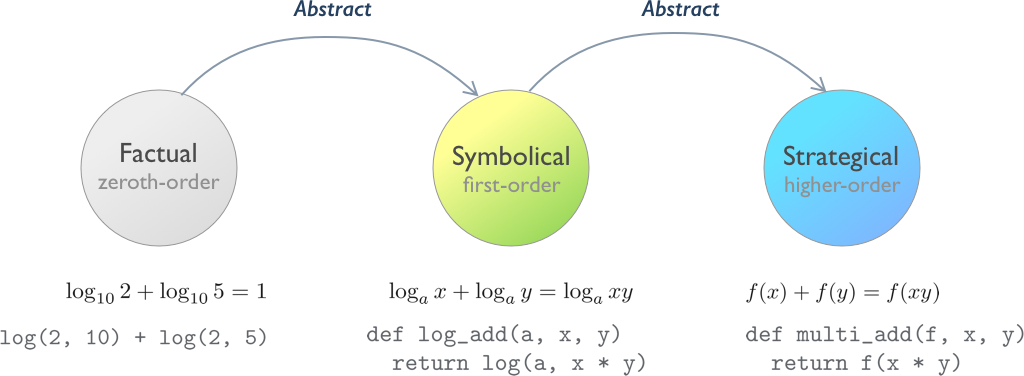
\includegraphics[width=\linewidth]{img/abstract-levels.png}
  \caption{Abstraction Levels}
  \label{fig:abstract-levels}
\end{figure}
\subsection{Robustness of Techniques}
\subsection{Frequency of Usage}
\subsection{Ad-Hoc versus Generic}
One phenominon that I experience a lot is the way people don't distinguish the difference between a ad-hoc technique and a generic technique. When a teacher or a guy present a way to solve a specific problem, few people will appreciate the robustness of this technique, that how well can you transfer your ability on this learning to another situations. But because of their inability to distinguish hardness and robustness, that leads to a dangerous place, that you have to learn too much techniques to cope with every problems, but you don't have enough time for learning these. And the teacher may think by doing an ad-hoc problem will lead to a better understanding for a more generic solving ability, which is vague. You don't learn too much on ad-hoc problems. You only know how to solve it in a nearby situations. The overall hint on a more generic solving strategies are often weak to recognize.

People don't know how to appreciate the robustness of techniques. Only can they find the dramatic changes of events. Even you simply press the button, you believe the underlining changes belongs to your smartness, well the main reason is the engineering behind the scene to smooth the user experience.
\subsection{Intensity of Signal}
\subsection{Trainability of Techniques}
Both the solving radius and the applicability.

% types of techniques
\section{Types of Techniques}
\subsection{Factual Techniques}
\subsection{Algorithmic Techniques}
\subsection{Strategic Techniques}
\subsection{Generic Techniques}
\subsection{Expansion Techniques}

% \section{Possible Hidden Places}
\subsection{Solve Like a Fox}
Don't try to generalize too early, and don't try to be perfect early on. The reason is simple, the cost is too much and the resource is limited. We can explore everything and make perfect choice at each step, the only way we could do is moving along. The wisdom is not even doing your best but to do the thing you can do, making progress instead of waiting for the right time or making the perfect match to your problem.

You can come up an idea and try it, then modify it later, and even you are improving it by visiting it multiple times. This strategy is simple but maybe powerful. It released the tension of limited resources. And it guesses along or maybe even believe its own ability that the result is at the reach and improve its understanding (I should define this word more precisely) along the way.

Solving a problem with ad hoc techniques may give the first hint of generalizations. But this route might be easier using the brutal force method rather the abst ract way thinking. We'd better revist the problem after solving, which will be a separate topic in the future.

The way of heuristics works in this book is that: in the indistinguishable path choosing situation, by assuming something may work,

\subsection{Increase the Similiarity}

\begin{example}
  If $2a+2^a = 5, 2b+ 2\log_2{(b-1)} = 5$, what is $a+b$?
\end{example}

You can solve $a$, which is around $1.28315$, and you can also get $b$, approximately $2.21685$. And the addition of these two numbers is exactly $3.5$. The important part of the transformation is to change the first part to $2a + 2 \cdot 2^{a-1} = 5$, so the two expression can have a symmetric look.

\chapter{Problems}

% introduction
\section{Problems}

To define a problem is defining a class at the same time.

To understand a problem is to know how to check whether one solution is correct or not.
\subsection{Verifying versus Searching}


% types of problems
\section{Types of Problems}
\subsection{Computational Problems}
\subsection{Learning Problems}
\subsection{Generic Problems}

% definition and properties of techniques
\section{Techniques}
The Classification of Techniques is a core concept in daily life.
\begin{figure}
  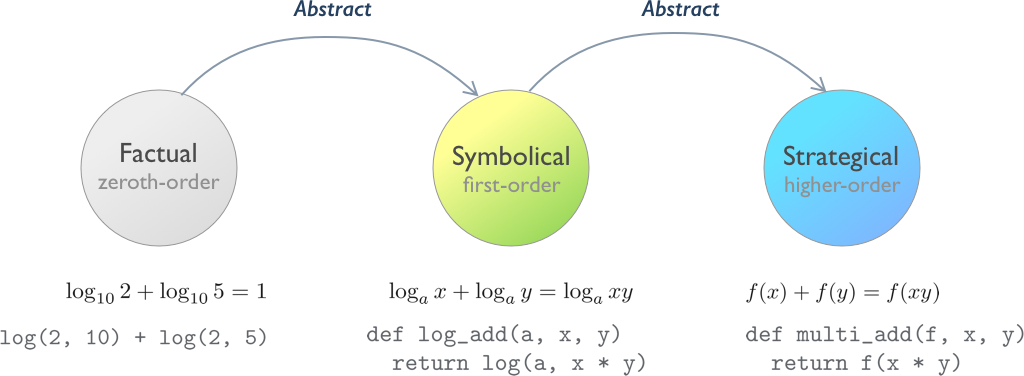
\includegraphics[width=\linewidth]{img/abstract-levels.png}
  \caption{Abstraction Levels}
  \label{fig:abstract-levels}
\end{figure}
\subsection{Robustness of Techniques}
\subsection{Frequency of Usage}
\subsection{Ad-Hoc versus Generic}
One phenominon that I experience a lot is the way people don't distinguish the difference between a ad-hoc technique and a generic technique. When a teacher or a guy present a way to solve a specific problem, few people will appreciate the robustness of this technique, that how well can you transfer your ability on this learning to another situations. But because of their inability to distinguish hardness and robustness, that leads to a dangerous place, that you have to learn too much techniques to cope with every problems, but you don't have enough time for learning these. And the teacher may think by doing an ad-hoc problem will lead to a better understanding for a more generic solving ability, which is vague. You don't learn too much on ad-hoc problems. You only know how to solve it in a nearby situations. The overall hint on a more generic solving strategies are often weak to recognize.

People don't know how to appreciate the robustness of techniques. Only can they find the dramatic changes of events. Even you simply press the button, you believe the underlining changes belongs to your smartness, well the main reason is the engineering behind the scene to smooth the user experience.
\subsection{Intensity of Signal}
\subsection{Trainability of Techniques}
Both the solving radius and the applicability.

% types of techniques
\section{Types of Techniques}
\subsection{Factual Techniques}
\subsection{Algorithmic Techniques}
\subsection{Strategic Techniques}
\subsection{Generic Techniques}
\subsection{Expansion Techniques}


\section{Variable-Based Strategies}
\subsection{Completeness of Information}

\section{Trial-Based Induction}

\section{Multi-Layer Exploration}

\section{The Generic Solving Algorithm}
\subsection{Frequecy of Usage}
\subsection{Comfort of Familiarness}
\subsection{Toolbox Hierarchy}
Analogy of a memory hierarchy.
\subsection{Automatic Exploration}

\section{Reviewing the Solution}
\subsection{Hardness of a Problem}
\subsection{Evaluation of the Solution}
\subsection{Improvements of the Solution}
\subsection{Improvements of the Solving Ability}

% Real World Problems
% Not sure should I include these.
\chapter{Problems}

% introduction
\section{Problems}

To define a problem is defining a class at the same time.

To understand a problem is to know how to check whether one solution is correct or not.
\subsection{Verifying versus Searching}


% types of problems
\section{Types of Problems}
\subsection{Computational Problems}
\subsection{Learning Problems}
\subsection{Generic Problems}

% definition and properties of techniques
\section{Techniques}
The Classification of Techniques is a core concept in daily life.
\begin{figure}
  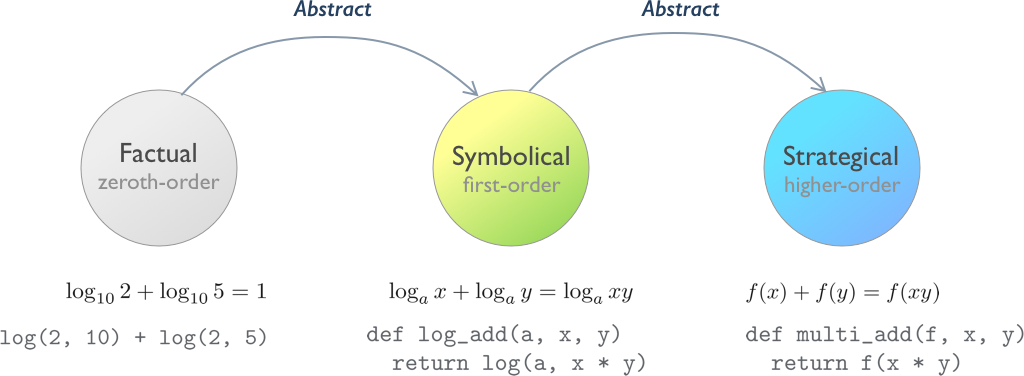
\includegraphics[width=\linewidth]{img/abstract-levels.png}
  \caption{Abstraction Levels}
  \label{fig:abstract-levels}
\end{figure}
\subsection{Robustness of Techniques}
\subsection{Frequency of Usage}
\subsection{Ad-Hoc versus Generic}
One phenominon that I experience a lot is the way people don't distinguish the difference between a ad-hoc technique and a generic technique. When a teacher or a guy present a way to solve a specific problem, few people will appreciate the robustness of this technique, that how well can you transfer your ability on this learning to another situations. But because of their inability to distinguish hardness and robustness, that leads to a dangerous place, that you have to learn too much techniques to cope with every problems, but you don't have enough time for learning these. And the teacher may think by doing an ad-hoc problem will lead to a better understanding for a more generic solving ability, which is vague. You don't learn too much on ad-hoc problems. You only know how to solve it in a nearby situations. The overall hint on a more generic solving strategies are often weak to recognize.

People don't know how to appreciate the robustness of techniques. Only can they find the dramatic changes of events. Even you simply press the button, you believe the underlining changes belongs to your smartness, well the main reason is the engineering behind the scene to smooth the user experience.
\subsection{Intensity of Signal}
\subsection{Trainability of Techniques}
Both the solving radius and the applicability.

% types of techniques
\section{Types of Techniques}
\subsection{Factual Techniques}
\subsection{Algorithmic Techniques}
\subsection{Strategic Techniques}
\subsection{Generic Techniques}
\subsection{Expansion Techniques}


% \section{Real-Life Solving}
% \subsection{Hierarchy of Human Needs}
% \subsection{Complexity of Human Aesthetic}
% \subsection{Sensibility of Human Aesthetic}
% \subsection{Alternative Reality}

\section{Designing the Solver}
\subsection{Benefits of the Solver}
\subsection{Revolution on the Foundation of Mathematics}
\subsection{Universal Algorithm of Distinguishability}
\subsection{Reinvent the Wheel}
\subsection{The End of Road}

The only problem we need to solve to solve all problems is the problem of problem solving.

So, why not solve it?
